\section{Evaluation}

In this section, we evaluate \name programs and report their contract profile
as well as illustrating the performance benefits of fine-grained consistency
classification on operations and transactions. We also report on the impact of
the summarization. We implemented the following applications, which includes
RDTs as well as larger applications composed of severals RDTs:

\begin{itemize} \item \textbf{LWW register}: A last-write-wins register. \item
\textbf{DynamoDB register}: A integer register that allows eventual and strong
puts and gets, conditional puts, increment and decrement operations. \item
\textbf{Bank account}: Our running example, with savings and current accounts.
\item \textbf{Shopping list}: Collaborative shopping list which allows adding
and deleting items. \item \textbf{Online store}: Models an online store with
shopping cart and dynamically changing item prices. Checkout process verifies
that the custormer only pays the accepted price. \item \textbf{RuBis}: An
ebay-like auction site~\cite{}. \item \textbf{Microblog}: A twitter-like
microblogging site, modelled after Twissandra~\cite{}. \end{itemize}

\subsection{Contract Characteristics}

\begin{table} \setlength{\tabcolsep}{4pt} {\sffamily \small \begin{center}
\begin{tabular} {|l|r|r|r|r|r|r|r|r|} \hline {\bf Benchmark} & {\bf LOC} & {\bf
\#T} & {\bf EC} & {\bf CC} & {\bf SC} & {\bf RC} & {\bf MAV} & {\bf RR} \\
\hline {LWW Reg} & 108 & 1 & 2 & 2 & 2 & 0 & 0 & 0 \\ {DynamoDB} & 126 & 1 & 3
& 1 & 2 & 0 & 0 & 0 \\ {Bank Account} & 155 & 1 & 1 & 1 & 1 & 1 & 0 & 1 \\
{Shopping List} & 140 & 1 & 2 & 1 & 1 & 0 & 0 & 0 \\ {Online store} & 340 & 4 &
9 & 1 & 0 & 2 & 0 & 1 \\ {Rubis} & 640 & 6 & 14 & 2 & 1 & 4 & 2 & 0 \\
{Microblog} & 659 & 5 & 13 & 6 & 1 & 6 & 3 & 1 \\ \hline \end{tabular}
\end{center} } \caption{The distribution of classfied contracts. \#T refers to
the number of tables in the application. The columns 4-6 (7-9) represent
operations (transactions) assigned to this consistency (isolation) level.}
\label{tab:ctrts} \end{table}

The distribution of contracts in these applications is given in
Table~\ref{tab:ctrts}. We see that majority of the operations are classified as
eventually consistent. Typically, causally consistent operations tend to be
reads that require to see operations in the same session or causally preceding
effects. Transactions are useful for maintaining cross-object consistency and
integrity constraints. For example, we maintain foregin key relationship
between tables using RC isolation level on the insertion transaction, and MAV
on the read transaction; if a MAV transaction witnesses the foreign key field
on table, then it \emph{will} witness the corresponding primiary key row in the
referenced table.

RR transaction comes in handy for maintaining the integrity of follow user
functionality in microblog. If user $A$ is followed by $B$, then we add a
\emph{followedBy} edge from $A$ to $B$ and a \emph{following} edge in the other
direction. The integrity constraint is that either both the edges are added, or
none. RR transaction isolation level is used to ensure correctness when
concurrently $A$ blocks $B$, and $B$ follows $A$. By operating on a snapshot of
consistent state, the block user transaction will not be interfered by the
concurrent follow user transaction.

The proof obligations associated with contract classfication is discarged
through the Z3 SMT Solver. In particular, the contract classification process
is completely performed compile time and has no overheads at runtime. Across
our benchmarks, classifying a contract took 11.5 milliseconds on average.

\subsection{Performance}

In this section, we study the performance benefit of fine-grained contract
classification, and the impact of summarization optimization.

\subsubsection{Configuration}

We deploy \name applications in \emph{clusters} where each cluster is composed
of 5 fully replicated Cassandra replicas within the same datacenter. We
instantiate one shim layer node for every cassandra replica, an place it on the
same VM as the cassandra replica. The clients are instantiated on the same data
center as the store, and run the transactions. We deploy the each node in the
cluster cluster on \cf{c3.4xlarge} Amazon EC2 instances with 16 virtual CPUs,
30GB memory, and 320GB of SSD storage. Our shim layer nodes are multi-threaded,
and we allocate 8 CPUs for each shim layer node. The clients also run on
\cf{c2.4xlarge} instances. We call this deployment \cf{1DC}. For our WAN
experiments, we instantiate 2 clusters (each with 5 nodes), one in US-east (N.
Virginia) and another in US-west (Oregon). The average latency between the
regions was 85 ms. We call this deployment \cf{2DC}.

\subsubsection{LWW Register}

\begin{figure*}
  \centering
  \subfigure[Operation performance 1DC]{\label{grf:LWW-perf-1DC}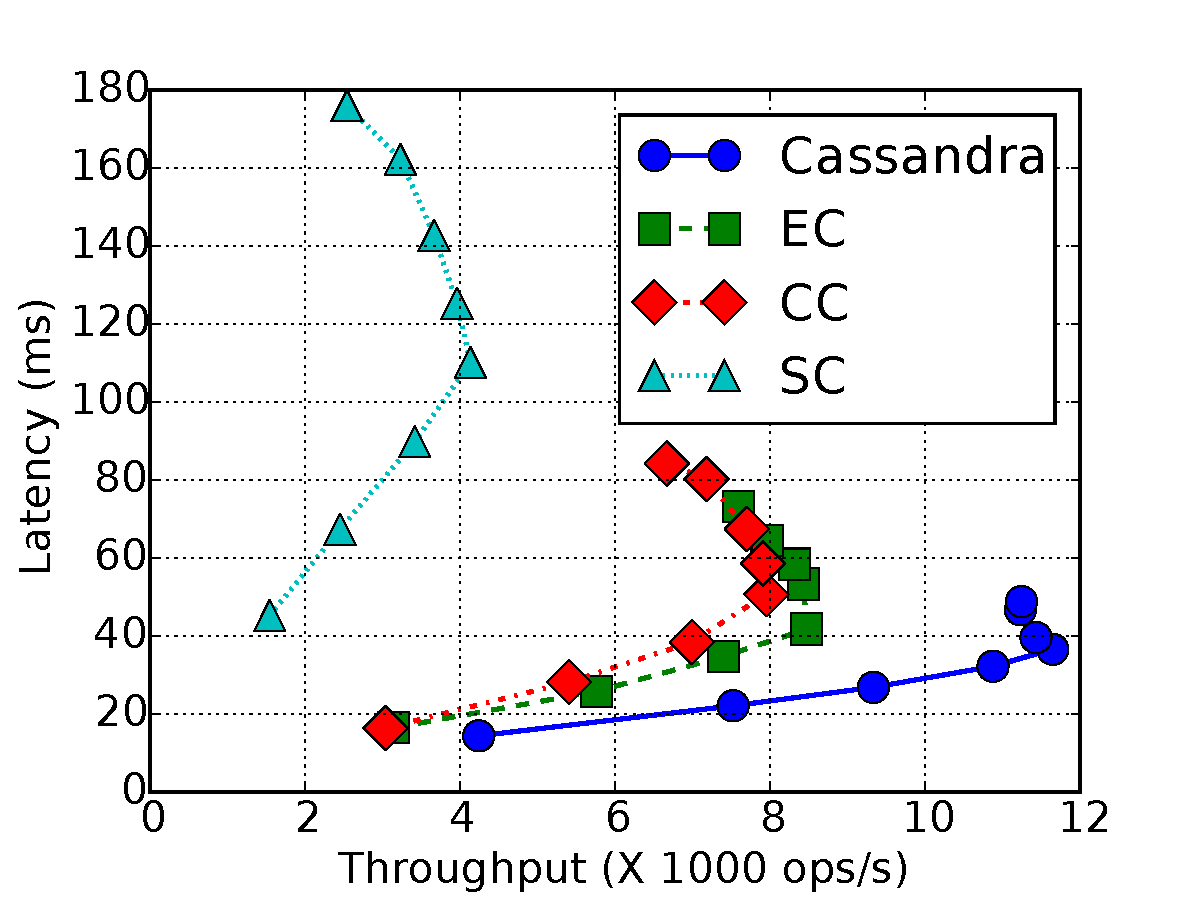
\includegraphics[width=0.24\textwidth]{graphs/LWW-tp-vs-lat-1DC.pdf}}
  \subfigure[Operation performance 2DC]{\label{grf:LWW-perf-2DC}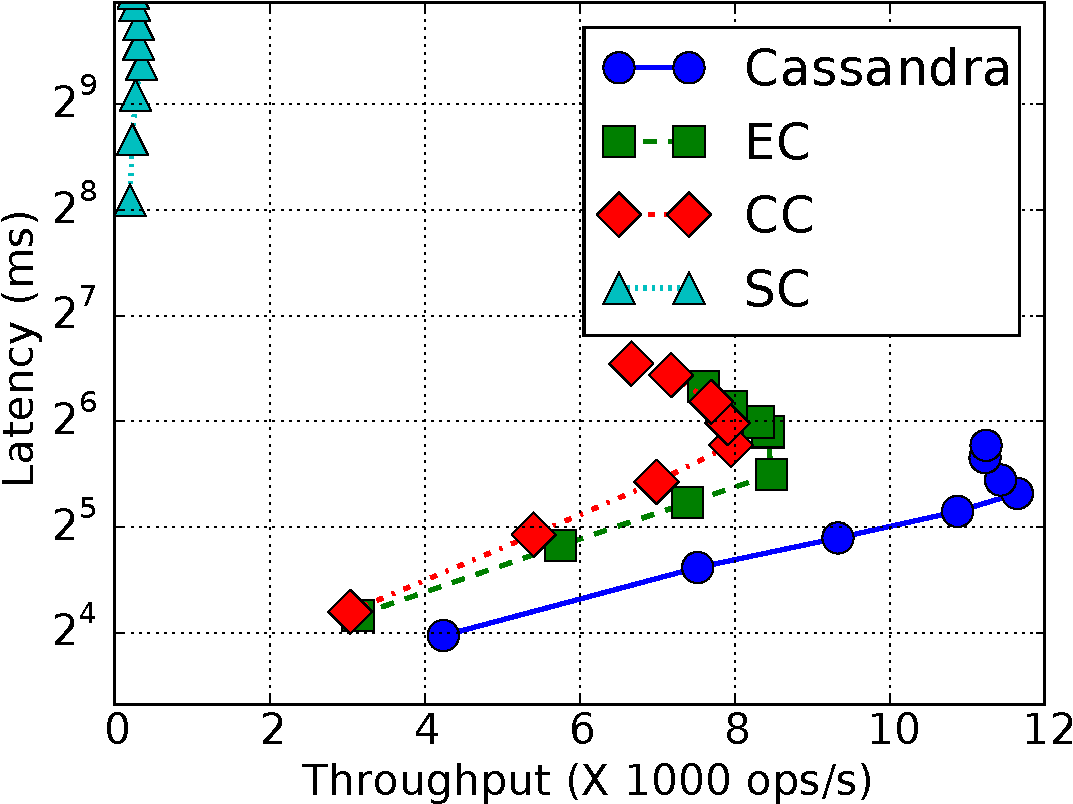
\includegraphics[width=0.24\textwidth]{graphs/LWW-tp-vs-lat-2DC.pdf}}
  \subfigure[Transaction performance 1DC]{\label{grf:LWW-txn-1DC}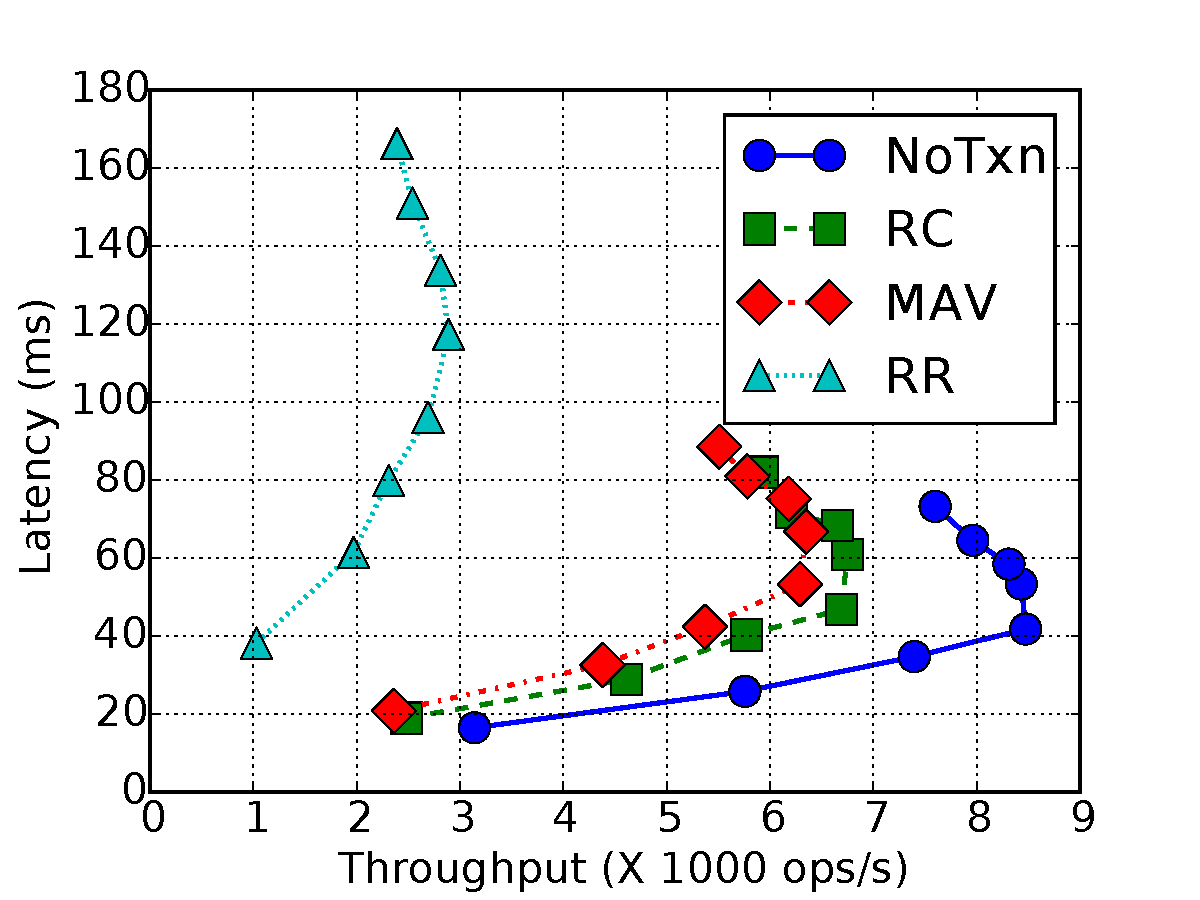
\includegraphics[width=0.24\textwidth]{graphs/LWW-tp-vs-lat-1DC-txn.pdf}}
  \subfigure[Mutations in transactions]{\label{grf:LWW-txn-wp}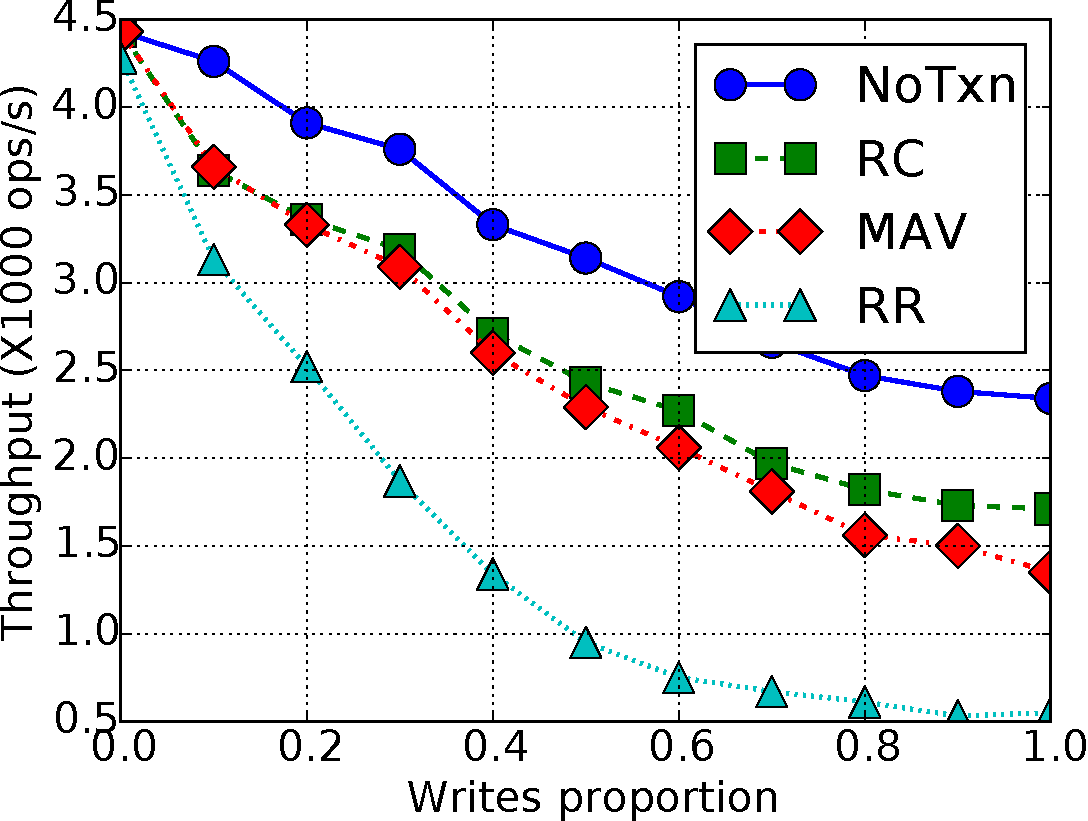
\includegraphics[width=0.24\textwidth]{graphs/LWW-txn-wp-vs-tp.pdf}}
	\caption{Performance of LWW Register RDT.}
  \label{grf:LWW_perf}
\end{figure*}

We analyze the performance of different consistency classifications in \name
using the LWW register. Our client workload was generated using YCSB
benchmark~\cite{}, with the default workload of 50\% reads and 50\% writes,
with keys uniformly chosen from a set of 100,000 keys. We varied the number of
clients from 128 to 1024, with each workload running for 180 seconds.
Last-writer-wins is the conflict resolution policy used by Cassandra. Hence, we
are able to directly compare the performance of \name implementation against
Cassandra.

Figure~\ref{grf:LWW-perf-1DC} shows the throughput vs. latency graph for the
different consistency levels in \cf{1DC} configuration. We also include
Cassandra, which provides basic eventual consistency. Recall that \name's
eventual consistency is stronger than the guarantees provided by Cassandra
(Section~\ref{sec:store_sem}). With 512 clients, the average latency of
operations on Cassandra was 32.24 milliseconds. EC and CC under \name was 30\%
and 57\% slower whereas strong consistency was 241\% slower. EC(SC) was able to
achieve 80\%(40\%) of throughput of vanilla Cassandra. The results show that
while \name provides an expressive programming model with stronger consistency
guarantees, its performance is comparable to vanilla Cassandra. However, SC has
a huge performance hit due to coordination between all the replicas for
obtaining object leases as well as reading and writing to all replicas. This
overhead worsens in a WAN setting. Figure~\ref{grf:LWW-perf-2DC} shows the
throughput vs. latency graph under 2DC configuration. While the Cassandra, EC
and CC numbers largely remain the same when compared to 1DC configuration, SC
is 6$\times$ to 12$\times$ higher latency and lower throughput than than the
1DC case.

We compare the performance of different transaction isolation level choices in
Figure~\ref{grf:LWW-txn-1DC}. The numbers were obtained under 1DC
configuration. The YCSB workload was modified to issue 10 operations per
transaction. Each operation is assumed to have eventual consistency. \cf{NoTxn}
corresponds to a configuration that does not use transactions. Compared to this
RC is only 12\% shower in terms of latency with 512 clients, where as RR is
2.3X slower. The difference between RC and \cf{NoTxn} is due to the meta-data
overhead of recording transaction information in the object state. For RR
transaction, The cost of capturing and maintaining the snapshot in an RR
transaction is the biggest source of overhead.

Moreover, the size of the snapshot is proportional to the the number of
different objects accessed by the session as well as the number of updates.
Hence, with increasing proportion of writes, the overhead of RR transaction
increases as shown in Figure~\ref{grf:LWW-txn-wp}. The numbers were obtained
with 128 clients. Compared to an RC transaction whose throughput decreasess
45\% as the write proportion increases from 0\% to 50\%, RR transaction's
throughput drops 78\% in the same interval.

\subsection{Bank Account}

\begin{figure}
  \centering
	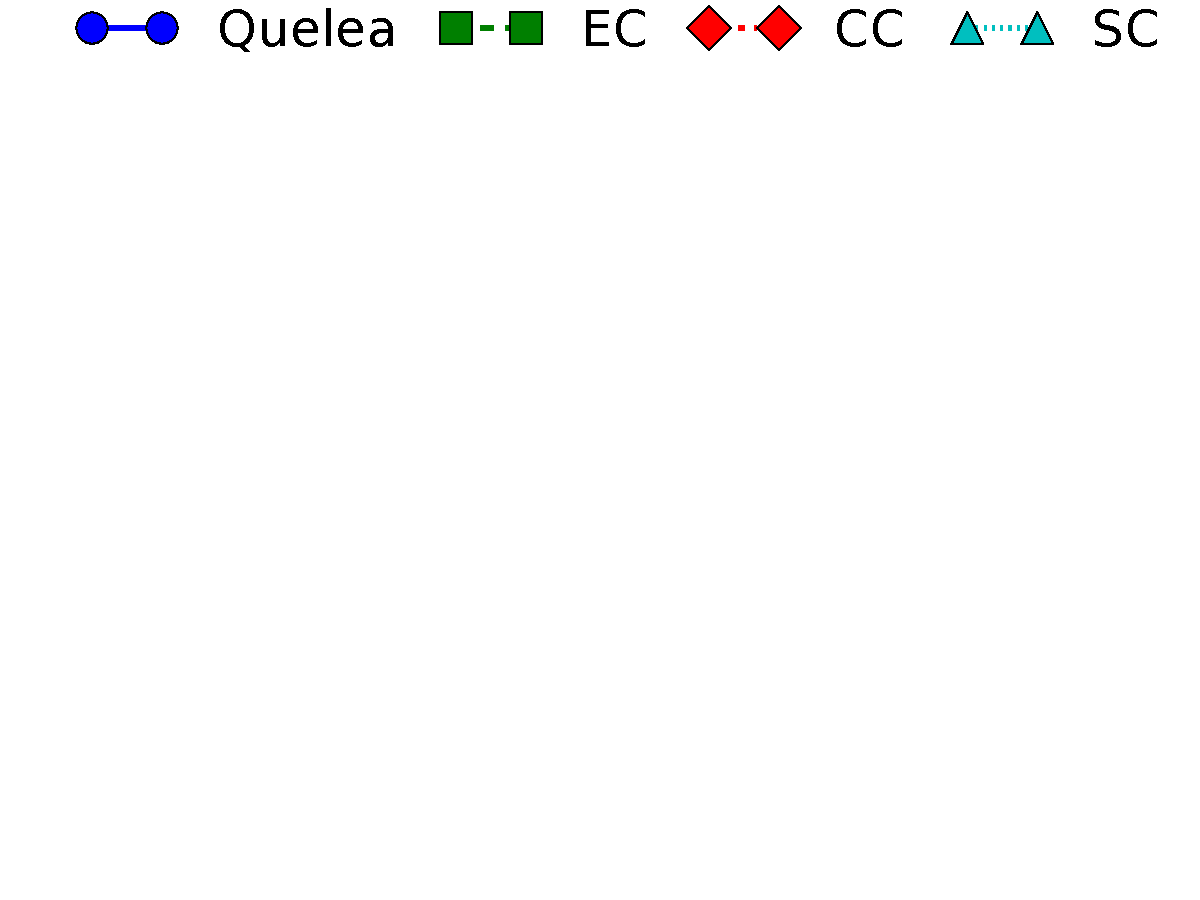
\includegraphics[width=0.5\columnwidth]{Figures/BA-legend.pdf}
  \subfigure[Latency 1DC]{\label{grf:BA-lat}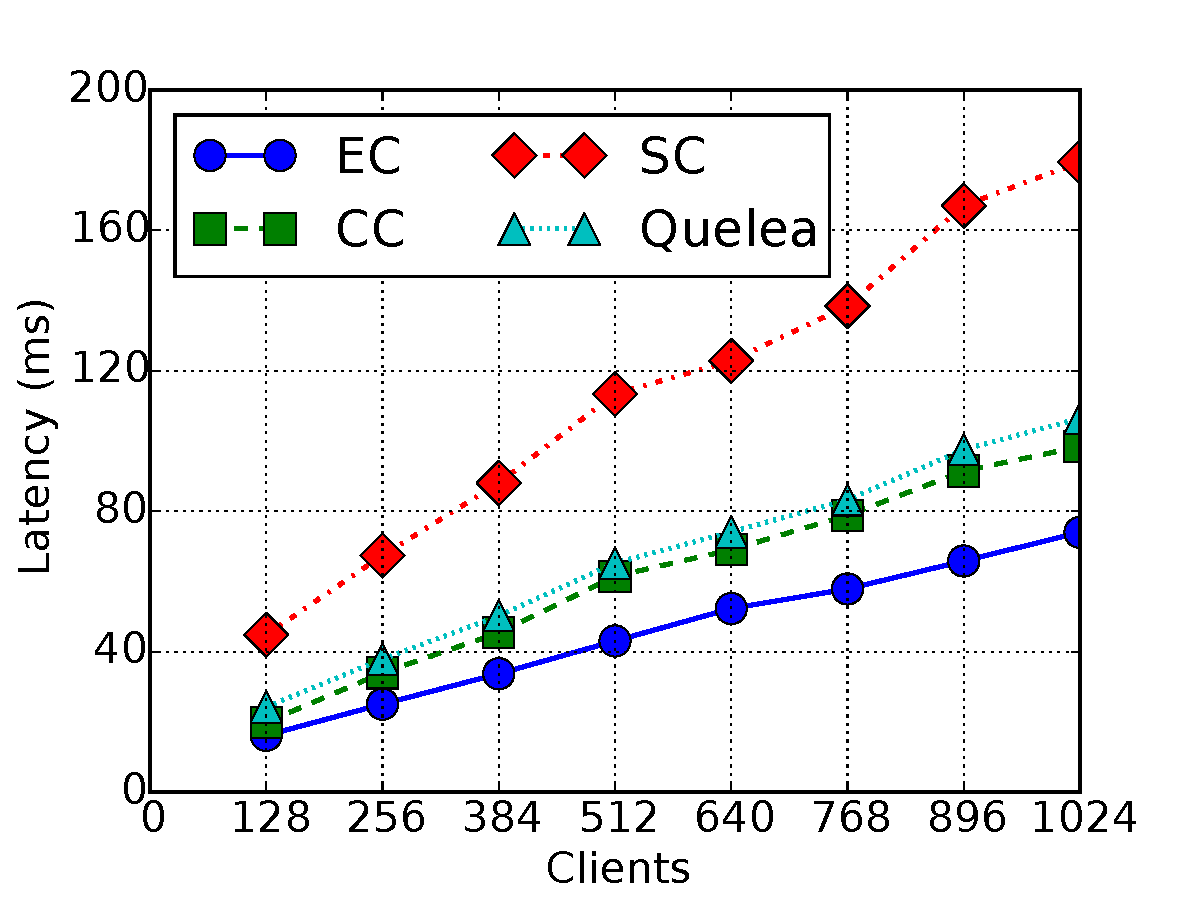
\includegraphics[width=0.24\textwidth]{graphs/BA-lat.pdf}}
  \subfigure[Throughput 1DC]{\label{grf:BA-tp}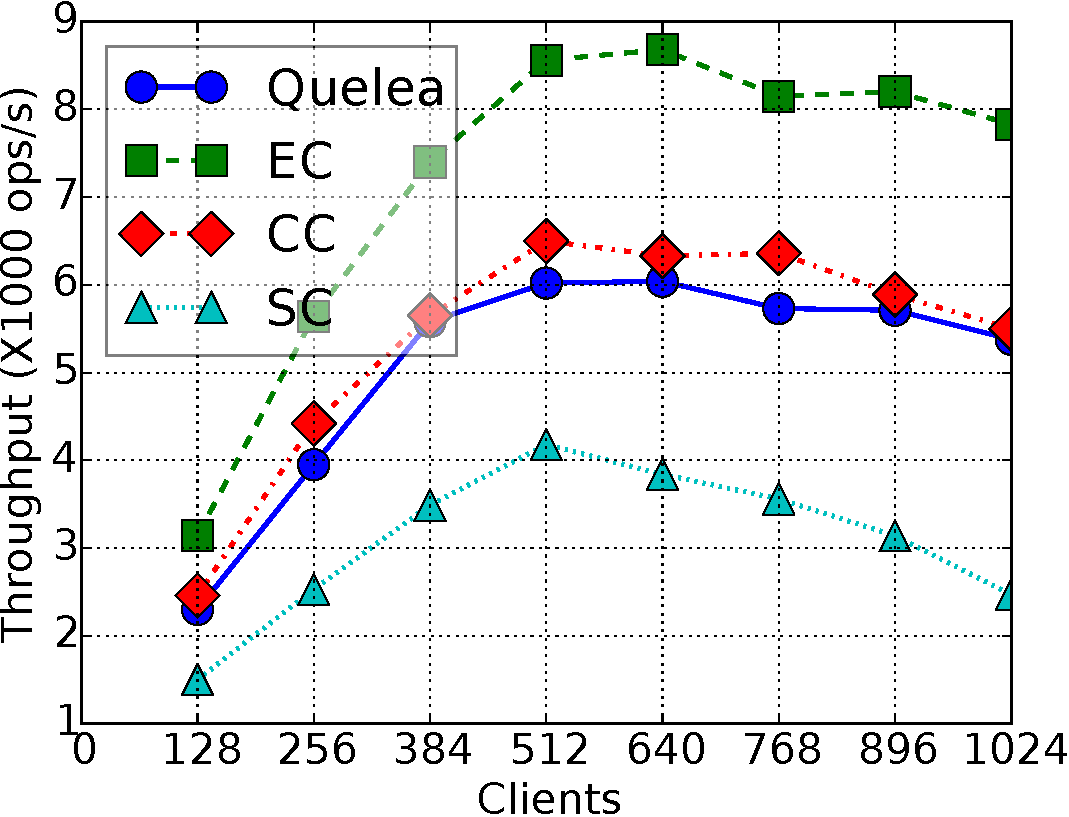
\includegraphics[width=0.23\textwidth]{graphs/BA-tp.pdf}}
	\caption{Performance of Bank Account RDT.}
  \label{grf:BA_perf}
\end{figure}

Figure~\ref{grf:BA-lat} and~\ref{grf:BA-tp} analyzes the latency and throughput
of operations in bank account example as we increase the number of clients in
\cf{1DC} configuration. The benchmark uniformly chose from 100,000 keys, where
the operation spread was 25\% withdraw, 25\% deposit and 50\% getBalance. Here,
the lines marked EC and CC correspond to all operations being assigned EC and
CC consistency levels. These levels compromise correctness as withdraw has to
be and SC operation. The line SC corresponds to a configuration where all
operations are strongly consistent; this ensures application correctness. \name
corresponds to our implementation, which classifies operations based on their
contracts. At 512 clients, \name implementation was within 30\% of latency and
12\% of throughput of EC, while providing correctness, whereas SC operations
had 162\% higher latency and 52\% lower throughput than EC operations. This
illustrates the benefit of fine-grained contract classification in \name.
